% !TEX program = xelatex
%%%%%%%%%%%%%%%%%%%%%%%%

\documentclass[11pt,aspectratio=169]{beamer} % 11pt is default
\usetheme{metropolis} % [progressbar=frametitle]
\setbeamercolor{background canvas}{bg=white}
\setbeamertemplate{caption}{\insertcaption} 
\setbeamersize{text margin left=2em,text margin right=2em}
\setbeamertemplate{frame footer}{\vspace{-5pt}}

\usepackage[round]{natbib}
\usepackage{amsmath}
\usepackage{mathtools}
\usepackage[group-minimum-digits=4,group-separator={,}]{siunitx}
\usepackage{graphicx}
\usepackage{wrapfig}
\usepackage{multimedia}

\usepackage{tikz}
\usetikzlibrary{backgrounds}
\usetikzlibrary{arrows,shapes}
\usetikzlibrary{tikzmark}
\usetikzlibrary{calc}
\usepackage[dvipsnames]{xcolor}

\usepackage[skins,theorems]{tcolorbox}
\usepackage{pdfpages}
\usepackage{colortbl}
\usepackage{changepage}
\usepackage{booktabs}
\usepackage{makecell}
\usepackage{setspace}
\usepackage{algorithm}
\usepackage[noend]{algpseudocode}
\usepackage{subcaption}
\usepackage[framemethod=TikZ]{mdframed}
\usepackage{xspace}

\usepackage{annotate-equations}

% Shortcut for beamer frames
\newcommand{\bframe}[2][c]{\begin{frame}[#1]{#2}}
\newcommand{\eframe}{\end{frame}} % \eframe causes problems for some reason

% Shortcut for bold text
\newcommand{\fat}[1]{\textbf{#1}}

% Boxing items on slide
\newcommand{\Cboxed}[2]{\colorlet{currentcolor}{.}{\color{#1}\fbox{\color{currentcolor}#2}}} %create coloured box around equation

% checkmark and xmark
\usepackage{pifont}
\newcommand{\cmark}{\ding{51}}%
\newcommand{\xmark}{\ding{55}}%

% Highlighting text in orange
\newcommand{\e}[1]{\alert{#1}}

% Underline
\newcommand{\uline}[1]{\underline{#1}}

% Include figure
\newcommand{\imgw}[2]{\includegraphics[width=#2\textwidth]{#1}} % \imgw{file}{height-scale}
\newcommand{\imgh}[2]{\includegraphics[height=#2\textheight]{#1}} % \imgh{file}{width-scale}

% Shortcut for latex commands
\newcommand{\blist}{\vspace{-3pt}\begin{list}{\raisebox{1pt}{\small$\bullet$}}{\leftmargin=13pt\itemsep=4pt}}
\newcommand{\blisttab}{\vspace{5pt}\blist}
\newcommand{\elisttab}{\end{list}}
\newcommand{\listtab}{\\[3pt] $\Rightarrow$ }
\newcommand{\elist}{\end{list}\vspace{5pt}}
\newcommand{\bblock}[1]{\metroset{block=fill}\begin{block}{#1}}
\newcommand{\eblock}{\end{block}}
\newcommand{\bmath}[1][0]{\begin{equation*}\hspace{#1em}}
\newcommand{\emath}{\end{equation*}}
\newcommand{\bcol}{\begin{columns}}
\newcommand{\col}[1]{\column{#1\textwidth}}
\newcommand{\tcol}[1]{\column[T]{#1\textwidth}}
\newcommand{\ecol}{\end{columns}}
\newcommand{\place}[4]{\begin{textblock}{#3}(#1,#2) #4 \end{textblock}} % \place{x}{y}{width}{text}
\newcommand{\placeframed}[4]{\place{#1}{#2}{#3}{\fbox{\parbox{#3em}{#4}}}}
\newcommand{\placeimg}[4]{\place{#1}{#2}{#3}{\imgw{#4}{1}}} % \placeimg{x}{y}{width}{file}
\newcommand{\videolink}[2]{\movie[externalviewer]{{\bf Video:} #1}{videos/#2}} % \videolink{title}{file}
\newcommand{\btab}[1]{\begin{tabular}{#1}}
\newcommand{\etab}{\end{tabular}}
\newcommand{\balgo}[2][1.3]{{#2:} \\[5pt] \begin{algorithmic}[1] \linespread{#1}\selectfont}
\newcommand{\ealgo}{\end{algorithmic}}
\renewcommand{\algorithmicloop}{\textbf{repeat:}}
\newcommand{\cred}{\cellcolor{red!25}}
\newcommand{\cgreen}{\cellcolor{green!25}}

% Shortcut for commonly used math symbols
\newcommand{\condpr}[2]{\text{Pr}\hspace{-1pt}\left\{ #1 \ \mid \ #2 \right\}}
\newcommand{\exarg}[2]{\mathbb{E}_{#1}\hspace{-2pt}\left[ #2 \right]}
\newcommand{\exnoarg}[1]{\mathbb{E}_{#1}}
\NewDocumentCommand\ex{ m g }{
	\IfNoValueTF{#2}{\exnoarg{#1}}{\exarg{#1}{#2}}
}
\newcommand{\der}[2]{\frac{\partial #1}{\partial #2}}
\newcommand{\stats}{\mathcal{S}}
\newcommand{\acts}{\mathcal{A}}
\newcommand{\rews}{\mathcal{R}}
\newcommand{\eps}{\mathcal{E}}
\newcommand{\ver}{\,\vert\,}
\newcommand{\vhat}{\hat{v}}
\newcommand{\qhat}{\hat{q}}
% \newcommand{\para}{\textbf{w}}
\newcommand{\feats}{\textbf{x}}
\newcommand{\elig}{\textbf{z}}
\newcommand{\gradient}{\nabla}
\newcommand{\outline}{Lecture Outline}
\newcommand{\reading}{Reading}
\newcommand{\h}[1]{\emph{#1}}

\emph
% \newcommand{\lindex}[1]{%
% 	\lowercase{\def\temp{#1}%
% 	\expandafter\index\expandafter{\temp}%
% }

\newcommand{\indx}[1]{\index{#1}}
\newcommand{\hind}[1]{\h{#1}\lindex{#1}}

% Set of real numbers
\newcommand{\R}{\mathbb{R}}
% Proportional to
% Transpose of a vector x
\newcommand{\vectranspose}[1]{#1^\top}
% Transpose of a matrix X
\newcommand{\mattranspose}[1]{#1^\top}
% Probability
\newcommand{\pr}{\text{Pr}}
% Conditional probability of x given y
\newcommand{\cpr}[2]{\pr( #1 \mid #2 )}
% x sampled according to probability distribution p
\newcommand{\sampled}[2]{#1 \sim #2}
% Assign value y to variable x
\newcommand{\assign}[2]{#1 \gets #2}
% Training data set
\newcommand{\data}{\mathcal{D}}
% Concatenation of inputs a, b, c, ...
\newcommand{\con}[1]{\langle #1 \rangle}
% array with bracket
\newcommand{\bra}[2]{\left[ \begin{array}{#1} #2 \end{array} \right]}
% Indicator function: returns 1 if x is true, otherwise returns 0
\newcommand{\ind}[1]{[#1]_1}

% common way of referring to places
\newcommand{\seehere}[1]{(\cref{#1})}

% shortcut text commands
\newcommand{\rl}{RL\xspace}
\newcommand{\marl}{MARL\xspace}
\newcommand{\ctde}{CTDE\xspace}
\newcommand{\sa}{single-agent\xspace}
\newcommand{\ma}{multi-agent\xspace}
\newcommand{\Ma}{Multi-agent\xspace}
\newcommand{\mas}{multi-agent system\xspace}
\newcommand{\stat}{stationarity\xspace}
\newcommand{\nonstat}{non-stationarity\xspace}
\newcommand{\pg}{policy gradient\xspace}
\newcommand{\vb}{value-based\xspace}
\newcommand{\pbt}{population-based training\xspace}
\newcommand{\psro}{policy space response oracles\xspace}
\newcommand{\Psro}{Policy space response oracles\xspace}
\newcommand{\sct}{\emph{StarCraft~II}\xspace}
\newcommand{\as}{AlphaStar\xspace}
\newcommand{\az}{AlphaZero\xspace}
\newcommand{\lbf}{level-based foraging\xspace}
\newcommand{\Lbf}{Level-based foraging\xspace}
\newcommand{\nfg}{normal-form game\xspace}
\newcommand{\nfgs}{normal-form games\xspace}
\newcommand{\Nfg}{Normal-form game\xspace}
\newcommand{\Nfgs}{Normal-form games\xspace}
\newcommand{\rps}{Rock-Paper-Scissors\xspace}
\newcommand{\pd}{Prisoner's Dilemma\xspace}
\newcommand{\survey}[4]{\noindent #1 (#4). ``#2.'' In: {\it #3}. \\}
\newcommand{\nashprob}{\textsc{Nash}\xspace}
\newcommand{\eol}{\textsc{End-of-Line}\xspace}
\newcommand{\ul}[1]{\underline{#1}}
\newcommand\norm[1]{\lVert#1\rVert}
\newcommand{\qlearn}{Q-learning\xspace}
\newcommand{\sarsa}{Sarsa\xspace}
\newcommand{\bayes}{Bayesian\xspace}
\newcommand{\bellman}{Bellman\xspace}
\newcommand{\markov}{Markov\xspace}
\newcommand{\pareto}{Pareto\xspace}
\newcommand{\boltzmann}{Boltzmann\xspace}
\newcommand{\mc}{Monte Carlo\xspace}
\newcommand{\nash}{Nash\xspace}
\newcommand{\ppad}{PPAD}
\newcommand{\dqn}{deep Q-networks\xspace}
\newcommand{\reinforce}{REINFORCE\xspace}
\newcommand{\qmix}{QMIX\xspace}
\newcommand{\qtran}{QTRAN\xspace}
\newcommand{\adam}{Adam\xspace}
\newcommand{\nret}{{$N$}-step returns\xspace}

% COMMANDS FOR COMMON NOTATION

% agent set
% state space
\newcommand{\St}{S}
\newcommand{\Stterm}{\bar{\St}}
% state
\newcommand{\st}{s}
\newcommand{\sth}{\hat{\st}}
% observation space
\newcommand{\Ob}{O}

% observation
\newcommand{\ob}{o}

% joint observation
\newcommand{\job}{o}
% action space
\newcommand{\Ac}{A}

% action
\newcommand{\ac}{a}
\newcommand{\ach}{\hat{\ac}}

% joint action
\newcommand{\jac}{a}
% reward
\newcommand{\rew}{r}
\newcommand{\rewh}{\hat{\rew}}
% centralised information
\newcommand{\ci}{z}

% initial state distribution

\newcommand{\instdist}{\mu}
% % state transition function

\newcommand{\Stf}{\mathcal{T}}
% % simulation/sampling model
\newcommand{\Stfsim}{\widehat{\Stf}}

% observation function
\newcommand{\Obf}{\mathcal{O}}

% reward function
\newcommand{\Rew}{\mathcal{R}}

% POLICIES, RETURNS, VALUES

% policy space
\newcommand{\Pol}{\Pi}

% policy
\newcommand{\pol}{\pi}
\newcommand{\poltil}{\tilde{\pol}}

% set of histories
\newcommand{\His}{H}
\newcommand{\Fhis}{\hat{\His}}
% history
\newcommand{\his}{h}

% full history
\newcommand{\fhis}{\hat{\his}}

% observation history extracted from full history
\newcommand{\obsext}{\sigma}

% discount factor
\newcommand{\dsc}{\gamma}

% return
\newcommand{\ret}{u}

% expected return for joint policy
\newcommand{\exret}{U}

% Agents
\newcommand{\Ag}{I}

% RL / MARL

% learning algorithm

\newcommand{\alg}{\mathbb{L}}

% empirical distribution/ average policy
\newcommand{\empdis}{\bar{\pol}}
\newcommand{\avgpol}{\bar{\pol}}
\newcommand{\agmod}{\hat{\pol}}
\newcommand{\Agmod}{\hat{\Pol}}
\newcommand{\agmodj}{agent model for agent $j$}

% best response
\newcommand{\br}{\textnormal{BR}}

% game value
\newcommand{\gval}{Value}

% value under agent model
\newcommand{\amval}{AV}

% regret
\newcommand{\regret}{Regret}
\newcommand{\avgreg}{\bar{R}}
% TD target
\newcommand{\target}{\mathcal{X}}
% step size (for gradient-based MARL in Chapter 5)
\newcommand{\step}{\kappa}


% DEEP LEARNING

% parameters
\newcommand{\para}{\theta}

% loss
\newcommand{\loss}{\mathcal{L}}
% batch
\newcommand{\batch}{\mathcal{B}}
\newcommand{\batchsize}{B}

% etnropy
\newcommand{\entropy}{\mathcal{H}}

% Create algorithm environment
\newcommand{\balg}[2]{
  \begin{algorithm}[H]
    \caption{#1}
    \label{alg:#2}
    \setstretch{1.1}
    \begin{algorithmic}[1]}

\newcommand{\ealg}{
    \end{algorithmic}
  \end{algorithm}}

% Argmin/ Argmax operators

\DeclareMathOperator*{\argmin}{arg\,min} 
\DeclareMathOperator*{\argmax}{arg\,max}

\makeatletter
\newenvironment{myitemize}{%
   \setlength{\topsep}{0pt}
   \setlength{\partopsep}{0pt}
   \renewcommand*{\@listi}{\leftmargin\leftmargini \parsep\z@ \topsep\z@ \itemsep\z@}
   \let\@listI\@listi
   \itemize
}{\enditemize}
\makeatother  

% define widebar for target parameters
\makeatletter
\newcommand*\rel@kern[1]{\kern#1\dimexpr\macc@kerna}
\newcommand*\widebar[1]{%
	\begingroup
	\def\mathaccent##1##2{%
		\rel@kern{0.8}%
		\overline{\rel@kern{-0.8}\macc@nucleus\rel@kern{0.2}}%
		\rel@kern{-0.2}%
	}%
	\macc@depth\@ne
	\let\math@bgroup\@empty \let\math@egroup\macc@set@skewchar
	\mathsurround\z@ \frozen@everymath{\mathgroup\macc@group\relax}%
	\macc@set@skewchar\relax
	\let\mathaccentV\macc@nested@a
	\macc@nested@a\relax111{#1}%
	\endgroup
}
\makeatother


% MATRIX GAMES

\newcolumntype{?}{!{\vrule width 1pt}}
\newcommand{\bhline}{\Xhline{1pt}}
\newcommand{\gametwo}[3]{
	\begin{tabular}{c?c|c}
		 & #1 \\
		\bhline
		#2    \\
		\hline
		#3    \\
	\end{tabular}
}
\newcommand{\gamethree}[4]{
	\begin{tabular}{c?c|c|c}
		 & #1 \\
		\bhline
		#2    \\
		\hline
		#3    \\
		\hline
		#4    \\
	\end{tabular}
}

\newcommand{\gamepd}{
    % \gametwo{C & D}{C & -1,-1 & -5,0}{D & 0,-5 & -3,-3}
	\begin{tabular}{c|c|c}
	& C & D \\
	\hline
	C & -1,-1 & -5,0 \\
	\hline
	D & 0,-5 & -3,-3
	\end{tabular}
}

\newcommand{\gamerps}{
    % \gamethree{R & P & S}{R & 0,0 & -1,1 & 1,-1}{P & 1,-1 & 0,0 & -1,1}{S & -1,1 & 1,-1 & 0,0}
	\begin{tabular}{c|c|c|c}
	& R & P & S \\
	\hline
	R & 0,0 & -1,1 & 1,-1 \\
	\hline
	P & 1,-1 & 0,0 & -1,1 \\
	\hline
	S & -1,1 & 1,-1 & 0,0
	\end{tabular}
}

\newcommand{\gamecoord}{
    % \gametwo{A & B}{A & 10 & 0}{B & 0 & 10}
	\begin{tabular}{c|c|c}
		& A & B \\
		\hline
		A & 10 & 0 \\
		\hline
		B & 0 & 10 \\
	\end{tabular}
}

\newcommand{\gamechicken}{
    % \gametwo{S & L}{S & 0,0 & 7,2}{L & 2,7 & 6,6}
	\begin{tabular}{c|c|c}
		& S & L \\
		\hline
		S & 0,0 & 7,2 \\
		\hline
		L & 2,7 & 6,6
	\end{tabular}
}

\newcommand{\gamestaghunt}{
    % \gametwo{S & H}{S & 4,4 & 0,3}{H & 3,0 & 2,2}
	\begin{tabular}{c|c|c}
		& S & H \\
		\hline
		S & 4,4 & 0,3 \\
		\hline
		H & 3,0 & 2,2
	\end{tabular}
}

\newcommand{\gamebattle}{
    \begin{tabular}{c|c|c}
    & A & B \\
    \hline
    A & 10,7 & 2,2 \\
    \hline
    B & 0,0 & 7,10
    \end{tabular}
}

\newcommand{\gameepsne}{
    % \gametwo{C & D}{A & 100,100 & 0,0}{B & 1,2 & 1,1}
	\begin{tabular}{c|c|c}
		& C & D \\
		\hline
		A & 100,100 & 0,0 \\
		\hline
		B & 1,2 & 1,1
	\end{tabular}
}

% Define colorboxes
\tcbset{
  % Defaults
  my box/main style/.style={},
  my box/title style/.style={},
  % Use the 'append' variants if you want to add to the defaults instead of
  % overriding them.
  my box/main/.style={/tcb/my box/main style/.style={#1}},
  my box/title/.style={/tcb/my box/title style/.style={#1}},
  my box/append main/.style={/tcb/my box/main style/.append style={#1}},
  my box/append title/.style={/tcb/my box/title style/.append style={#1}},
  %
  my box/.style={
    my box/.cd, #1,
    /tcb/.cd,
    enhanced,
    my box/main style,
    attach boxed title to top left={xshift=0.2cm, yshift=-0.2cm},
    top=10pt,
    boxed title style={
      outer arc=0pt,
      arc=0pt,
      top=3pt,
      bottom=3pt,
      my box/title style,
    },
  },
}

% define 'solutionbox' environment with coloured box
\newtcolorbox{solutionbox}[1][]{
  my box={
    main={colframe=green!40!gray!90, colback=green!20!gray!5},
    title={colback=green!40!gray!90},
  },
  title=Solution,
  #1,
}

\newtcolorbox{problembox}[1][]{
  my box={
    main={colframe=red!40!gray!90, colback=red!20!gray!5},
    title={colback=red!40!gray!90},
  },
  title=Problem,
  #1,
}

\newtcolorbox{notebox}[1][]{
  my box={
    main={colframe=orange!40!gray!80, colback=orange!20!gray!5},
    title={colback=orange!40!gray!80},
  },
  title=Note,
  #1,
}

\newtcolorbox{intuitionbox}[1][]{
  my box={
    main={colframe=blue!60!gray!80, colback=blue!20!gray!5},
    title={colback=blue!60!gray!80},
  },
  title=Intuition,
  #1,
}

\newtcolorbox{reminderbox}[1][]{
  my box={
    main={colframe=black!40!gray, colback=gray!10!white},
    title={colback=black!40!gray},
  },
  title=Reminder,
  #1,
}

\newtcolorbox{custombox}[2][]{
  my box={
    main={colframe=black!40!gray, colback=gray!10!white},
    title={colback=black!40!gray},
  },
  title={#2},
  #1,
}

% no title boxes
\newtcolorbox{greenbox}[1][]{
  my box={
    main={colframe=green!40!gray!90, colback=green!20!gray!5},
  },
  #1,
}
\newtcolorbox{redbox}[1][]{
  my box={
    main={colframe=red!40!gray!90, colback=red!20!gray!5},
  },
  #1,
}
\newtcolorbox{orangebox}[1][]{
  my box={
    main={colframe=orange!40!gray!80, colback=orange!20!gray!5},
  },
  #1,
}
\newtcolorbox{bluebox}[1][]{
  my box={
    main={colframe=blue!60!gray!80, colback=blue!20!gray!5},
  },
  #1,
}
\newtcolorbox{blackbox}[1][]{
  my box={
    main={colframe=black!55!black, colback=gray!5!white},
  },
  #1,
}


% Define intro slide command
\newcommand{\introslide}{
    \begin{frame}{MARL Book}
        \begin{columns}
            \begin{column}{0.5\textwidth}
            \begin{figure}
              \centering
              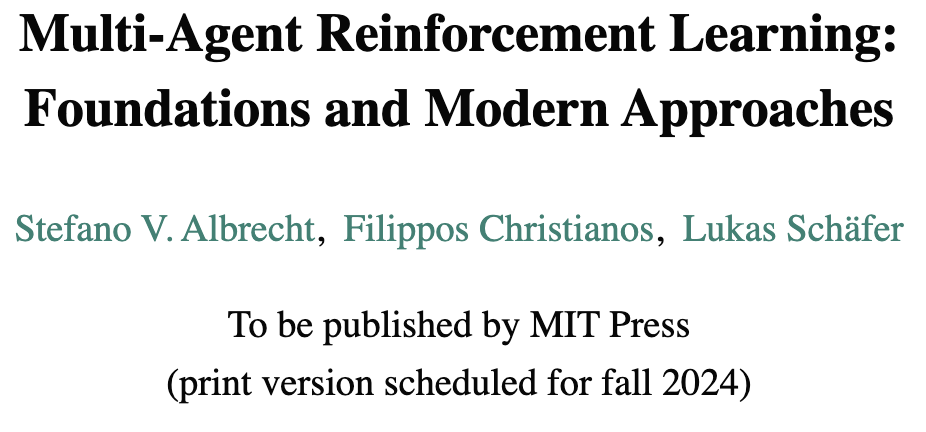
\includegraphics[width=\textwidth,height=.8\textheight,keepaspectratio]{images/1_MARL_book.png}
            
              \label{fig:enter-label}
            \end{figure}
          \end{column}
        
        \hspace{20pt}
            
          % Column for the text
            \begin{column}{0.45\textwidth}
	        \small

                This lecture is based on \textit{Multi-Agent Reinforcement Learning: Foundations and Modern Approaches} by Stefano V. Albrecht, Filippos Christianos and Lukas Sch\"afer
                
                \vspace{20pt}
                
                The book can be downloaded for free at \textcolor{blue}{\href{https://www.marl-book.com/}{www.marl-book.com}}.
            \end{column}
        
        \end{columns}
    \end{frame}
}

\newcommand{\leoslide}{
  \author{Stefano V. Albrecht, Filippos Christianos, Lukas Sch\"afer \\ Slides by: Leonard Hinckeldey}
}

\newcommand{\otherslide}{
  \author{Stefano V. Albrecht, Filippos Christianos, Lukas Sch\"afer}
}
	
\title{Multi-Agent Reinforcement Learning}
\date{}

\hypersetup{
  pdfsubject = {Multi-Agent Reinforcement Learning},
}

\leoslide

\subtitle{Games: Models of Multi-Agent Interaction}

\begin{document}
\maketitle

\introslide

\begin{frame}{\outline}
    \vspace{10pt}
    \fat{Part 1: Game Models} 
    \vspace{5pt}
    \blist
        \item Normal-form games
        \item Stochastic games
        \item Partially observable stochastic games  
    \elist
    \fat{Part 2: Modeling Communication} 
    \vspace{5pt}
    \blist
        \item Communication as an action
        \item Communication with observation functions
    \elist

    \fat{Part 3: Assumptions}
    \blist
        \item Game theory vs MARL assumptions
    \elist
\end{frame}

\section{Game Models}

\begin{frame}{Hierarchy of Games}

    % \begin{columns}
    % \begin{column}{0.3\textwidth}
    % Hierarchy from most to least general
    % \begin{enumerate}
    %     \item Partially observable stochastic Games (POSG)
    %     \item Stochastic games
    %     \item Normal-form games 
    % \end{enumerate}
    % \end{column}
    % \begin{column}{0.7\textwidth}
    \begin{figure}
        \centering
        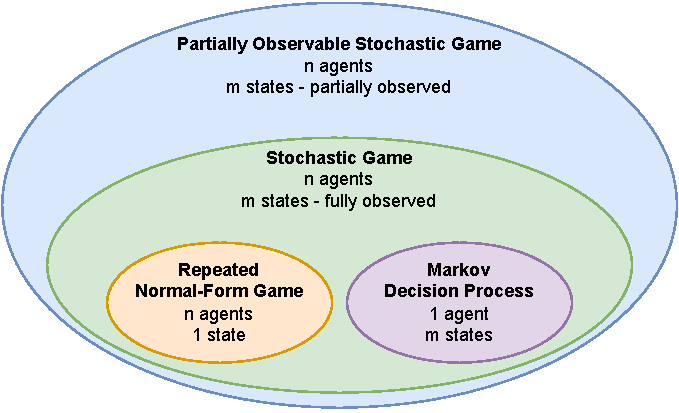
\includegraphics{images/chapter_3/game-hierarchy.pdf}
        \label{fig:enter-label}
    \end{figure}
    % \end{column}
    % \end{columns}
\end{frame}


\begin{frame}{Normal-Form Games}

    \fat{Normal-form} games define a \fat{single} interaction between two or more agents, providing a simple kernel for more general games to build upon. 
    \vspace{5pt}
    
    \pause
    
    \fat{Normal-form} games are defined as a 3 tuple \((I, \{A_i\}_{i \in I}, \{\mathcal{R}_i\}_{i \in I})\):
    \blist
        \item<2-> $I$ is a finite set of agents \(I = \{1, ..., n\}\)
        \item<3-> For each agent \(i \in I\):
        \blist
            \item \(A_i\) is a finite set of actions
            \item \(\mathcal{R}_i\) is the reward function \(\mathcal{R}_i: A \to \mathbb{R}\) where \(A = A_1 \times ... \times A_n\) (set of \fat{joint} actions). 
        \elist
    \elist
    
\end{frame}


\begin{frame}{Normal-Form Game Process}

    In a normal-form game, there are \fat{no time steps or states}. Agents choose an action and observe a reward.
    \vspace{10pt}
    
    \visible<1->The game proceeds as follows:
    \pause
    
    \begin{enumerate}
        \item<2-> Each agent samples an action \(a_i \in A_i\) with probability \(\pi_i(a_i)\)
        \pause
        \item<3-> The resulting actions from all agents form a \fat{joint action}, \(a = (a_1, ... , a_n)\)
        \pause
        \item<4-> Each agent receives a reward based on its \fat{individual} reward function and the \fat{joint action}, \(r_i = \mathcal{R}_i(a)\)
    \end{enumerate}
    
\end{frame}

\begin{frame}{Classes of Games}

    Games can be classified based on the relationship between the agents' reward functions. 

    \blist
        \item<1-> In \fat{zero-sum games}, the sum of the agents' reward is always 0\\
        i.e. \(\sum_{i \in I} \mathcal{R}_{i} (a) = 0, \forall a \in A\)

        \item<2-> In \fat{common-reward} games, all agents receive the same reward 
        (\(R_i = R_j ; \forall i, j \in I\))

        \item<3-> In \fat{general-sum} games, there are no restrictions on the relationship between reward functions. 
    \elist
    
\end{frame}

\begin{frame}{Matrix Games}

     Normal-from games with \fat{2} agents are also called \fat{matrix games} because they can be represented using reward matrices.

    \vspace{10pt} 
    
        \centering
        \begin{minipage}[b]{0.32\textwidth}
            \centering
            \gamerps
            
            \vspace{5pt}
            Rock-Paper-Scissors
            \onslide<2->{zero-sum} % Appears beneath the first minipage
        \end{minipage}\hfill
        \begin{minipage}[b]{0.32\textwidth}
            \centering
            \gamecoord
            
            \vspace{5pt}
            Coordination Game
            % \setcounter{enumi}{1} % Continue enumeration
            \onslide<3->{common-reward} % Appears beneath the second minipage
        \end{minipage}\hfill
        \begin{minipage}[b]{0.32\textwidth}
            \centering
            \gamepd
            
            \vspace{5pt}
            Prisoner's Dilemma
            \onslide<4->{general-sum} % Appears beneath the third minipage
        \end{minipage}

\end{frame}

\begin{frame}{Repeated Normal-Form Games}

\begin{figure}
    \centering
    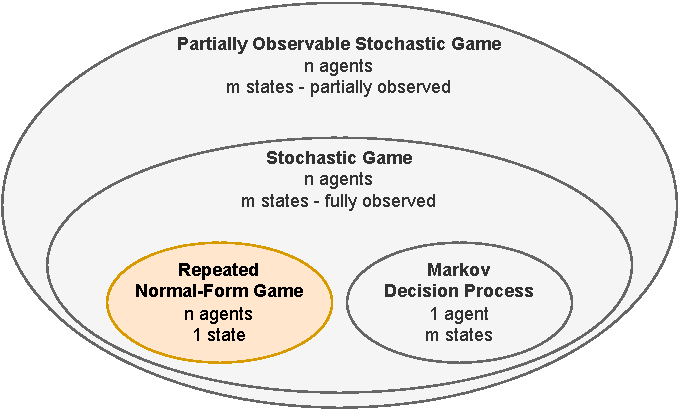
\includegraphics{images/chapter_3/normal_form_hierarchy.pdf}
    % \caption{Caption}
    % \label{fig:enter-label}
\end{figure}
    
\end{frame}


\begin{frame}{Repeated Normal-Form Games}

To extend normal-form games to \fat{sequential} multi-agent interaction, we can repeat the same game over \(T\) timesteps. 

    \begin{columns}
    \begin{column}{0.4\linewidth}
    \begin{figure}
        \centering
        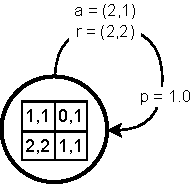
\includegraphics{images/chapter_3/game-models-mg.pdf}
        \label{fig:enter-label}
    \end{figure}
    \end{column}

    \begin{column}{0.6\linewidth}

    \blist
        \item At each time step \(t\) an agent $i$ samples an action \(a^{t}_{i}\)
        \item The policy is now conditioned on a \fat{joint-action} history \(\pi_i(a_{i}^{t}|h^t)\) where \(h^t = (a^o, ..., a^{t-1})\)
        \item In special cases, $h^t$ contains $n$ last joint actions. E.g. in a tit-for-tat strategy (Axelrod and Hamilton 1981), the policy is conditioned on \(a^{t-1}\)
    \elist
        
    \end{column}
    \end{columns}
\end{frame}

\begin{frame}{Stochastic Games}

\begin{figure}
    \centering
    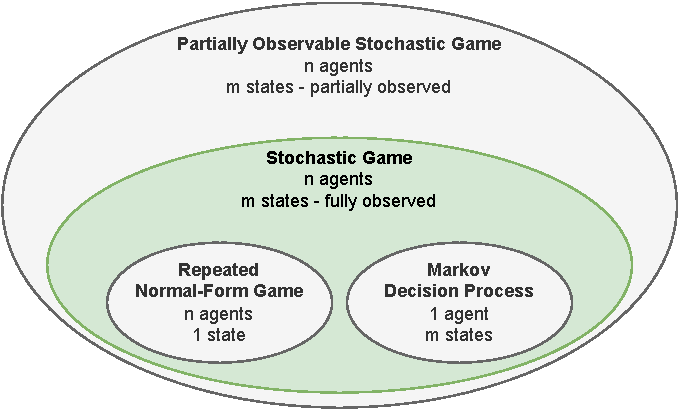
\includegraphics{images/chapter_3/stochastic_games_hierarchy.pdf}
    % \caption{Caption}
    % \label{fig:enter-label}
\end{figure}
\end{frame}

\begin{frame}{Stochastic Games}

    \e{\bf Stochastic games} introduce the notion of \fat{states} and are defined as a 6 tuple \((I, S, \{A_i\}_{i \in I}, \{\mathcal{R}_i\}_{i \in I}, \mathcal{T}, \mu)\)
    \vspace{10pt}
    \blist
        \item<2-> $I$ is a finite set of agents
        \item<3-> $S$ is a finite set of states with subset of terminal states $\bar{S} \subset S$
        \item<4-> For each agent $i \in I$:
        \blist
            \item $A_i$ is a set finite set of actions
            \item $\mathcal{R}_i$ is the reward function $\mathcal{R}_i : S \times A \times S \to \mathbb{R}$ where $A$ is the set of \fat{joint} actions $A = A_1 \times ... \times A_n$
        \elist
        \item<5-> $\mathcal{T}$ is the state transition function $\mathcal{T}: S \times A \times S \to [0, 1]$
        \item<6-> $\mu$ is the initial state distribution $\mu: S \to [0, 1]$
    \elist

\end{frame}


\begin{frame}{Stochastic Games - Continued}
    
    \begin{columns}
    \begin{column}{0.5\linewidth}
    \begin{figure}
        \centering
        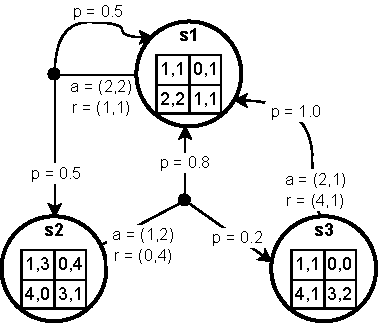
\includegraphics{images/chapter_3/game-models-sg.pdf}
        \label{fig:enter-label}
    \end{figure}
    \end{column}
    \vspace{10pt}
    \begin{column}{0.5\linewidth}

    \blist
        \item Each \fat{state} can be viewed as a \fat{non-repeated normal-form game}
        \item Stochastic games can also be classified into: zero-sum, common-reward or general-sum
        \item The figure on the left shows a general-sum case 
    \elist
        
    \end{column}
    \end{columns}
\end{frame}

\begin{frame}{Stochastic Game Process}

\begin{enumerate}
    \item<1-> Initial state $s_0 \in S$ is samples from $\mu$.
    \item<2-> At time $t$ each agent $i \in I$ observes the current state $s^{t} \in S$ and chooses an action $a^{t}_i \in A_i$ with probability $\pi_i(a^{t}_i|h^{t})$ 
    \vspace{2pt}
    \blist
        \item<3-> $h^t = (s^0, a^0, s^1, a^1, ......, s^t)$ is the \fat{state-action history} containing the current state $s^t$ and past \fat{joint} actions and states
    \elist
    \vspace{2pt}
    \item<4-> Given $s^t$ and $a^t$, the game transitions into the next state $s^{t+1} \in S$ with probability $\mathcal{T}(s^{t+1}|s^t, a^t)$
    \item<5->  Each agent receives a reward according to their reward function $r^{t}_{i} = \mathcal{R}_{i} (s^t, a^t, s^{t+1})$ 
    \item<6-> These steps are repeated until a terminal state $s^t \in \bar{S}$ is reached or a maximum number of T time steps is completed
\end{enumerate}
\end{frame}



\begin{frame}{Example: Level-Based Foraging}

\begin{columns}
    \begin{column}{0.45\textwidth}
    \begin{figure}
        \centering
        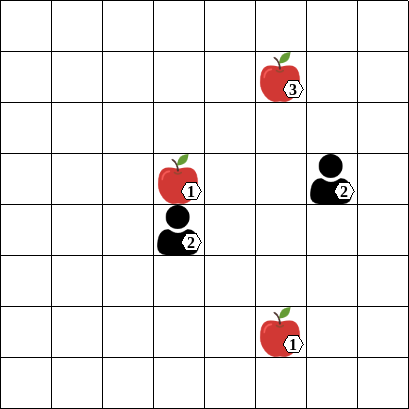
\includegraphics[width = 0.8\linewidth, keepaspectratio]{images/environments/lbf/lbf-8x8-2p-3f.png}
        \label{fig:enter-label}
    \end{figure}
    \end{column}

    \begin{column}{0.55\textwidth}
    \vspace{5pt}
    \blist
        \item \(s \in S\): vector of x-y positions for agents/items, binary collection flags, levels for agents/items
        \item \(a_i \in A_i\): move in four directions, collect item, or no operation (noop)
        \item \(\mathcal{T}\): joint actions update state, e.g., two agents collecting an item switch its flag
        \item \(\mathcal{R}\):
            \blist
                \item common-reward: +1 reward for any item collected by any agent
                \item general-sum: +1 reward only for agents directly involved in item collection
            \elist
    \elist
    \end{column}

\end{columns}
\end{frame}

\begin{frame}{Partially Observable Stochastic Games (POSG)}

\begin{figure}
    \centering
    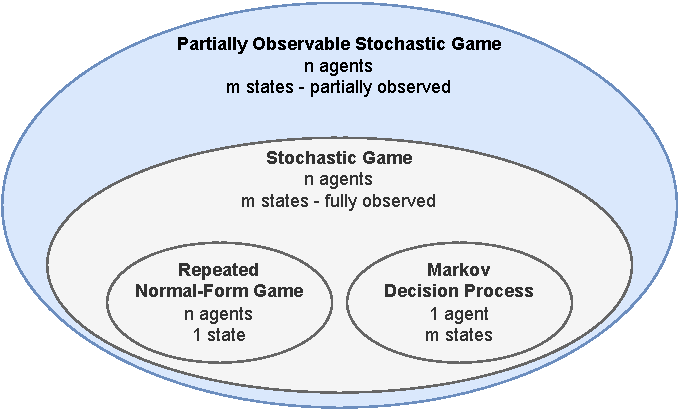
\includegraphics{images/chapter_3/POSG_hierarchy.pdf}
    % \caption{Caption}
    % \label{fig:enter-label}
\end{figure}
    
\end{frame}

\begin{frame}{Partially Observable Stochastic Games (POSG)}
    At the top of the game model hierarchy, the most \fat{general} model is the POSG
    \blist
        \item POSGs represent complex decision processes with \fat{incomplete information}
        \item Unlike in stochastic games, agents receive \fat{observations} providing \fat{incomplete information} about the state and agents' actions
        \item POSGs apply to scenarios where agents have limited sensing capabilities
       		\listtab e.g. autonomous driving
            \listtab e.g. strategic games (e.g. card games) with private, hidden information
    \elist
    
\end{frame}

\begin{frame}{POSG Definition}

POSG is defined in the same way stochastic games are, with two additions. Thus it is defined as a 8 tuple \((I, S, \{A_i\}_{i \in I}, \{\mathcal{R}_i\}_{i \in I}, \mathcal{T}, \mu, \e{\{O_{i}\}_{i \in I}, \{\mathcal{O}_{i}\}_{i \in I}})\)
\vspace{5pt}

\begin{columns}
    \begin{column}{0.5\textwidth}
    \begin{figure}
        \centering
        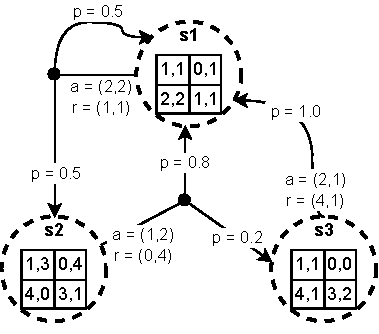
\includegraphics[width = 0.9\linewidth, keepaspectratio]{images/chapter_3/game-models-posg.pdf}
    \end{figure}
    \end{column}
    \begin{column}{0.5\textwidth}
        For each agent \(i\) we additionally define:
        \blist
            \item a finite set of observation \(O_{i}\)
            \item  an observation function $\{\mathcal{O}_{i}\}_{i \in I}$ such that $\mathcal{O}_i: A \times S \times O_i \to [0, 1]$ and $\forall a \in A, s \in S: \sum_{o_i \in O_i} \mathcal{O}_i (a, s, o_i) = 1$
        \elist
    \end{column}
\end{columns}
\end{frame}

\begin{frame}{POSG Process}

\begin{enumerate}
    \item<1-> Initial state $s^0$ sampled from $\mu(s)$
    \item<2-> At each $t$ every agent $i$ receives an \fat{observation} $o^{t}_{i} \in O_i$, with probability given by the observation function $\mathcal{O}_i(o^{t}|s^t, a^{t-1})$
    \item<3-> Each agent then chooses an action $a^{t}_{i}$ based on its policy $\pi_{i}$, which is conditioned on the agent's observation history, $h_{i} = (o^{0}_{i}, ..., o_{i}^{t})$. All agents' actions give the joint action $a^t = (a^{t}_{1}, ..., a^{t}_n)$
    \item<4-> Given the joint action, the environment transitions into the next state $s^{t+1}$ with probability $\mathcal{T}(s^{t+1}|s^t, a^t)$ and each agent receives a reward based on its reward function $r^{t}_{i} = \mathcal{R}_{i}(s^t, a^t, s^{t+1})$
    \item<5-> This is done until a terminating state $s^{t} \in \bar{S}$ is reached or a maximum number of time steps is completed
\end{enumerate}
    
\end{frame}

\begin{frame}{The Observation Function}

POSG can represent diverse observability conditions. For example:
\blist
    \item modeling noise by adding uncertainty in the possible observation
    \item to limit the visibility region of agents (see LBF example)
\elist

\vspace{10pt}

\bcol
    \col{0.5}
    	\centering
        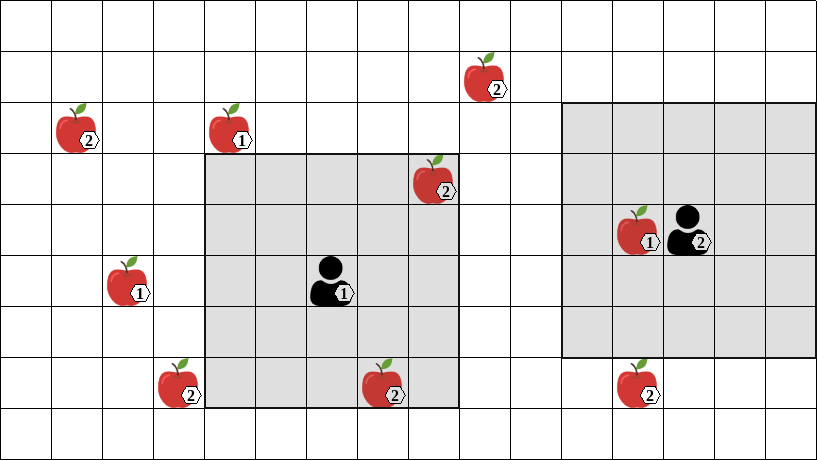
\includegraphics[width = 0.95\linewidth]{images/environments/lbf/foraging_po.png}
        
    \col{0.5}
        \blist 
            \item Here, the agent can only see some parts of the state and joint action
            \item \(o^{t}_{i} = (\bar{s}^t, \bar{a}^t)\) where \(\bar{s}^t \subset s^t, \bar{a}^t \subset a^t\)
        \elist
\ecol
\end{frame}

\begin{frame}{Belief States}

    In partially observable settings, it becomes more challenging to infer optimal actions. For example:

    \begin{columns}
    \begin{column}{0.6\textwidth}
    \vspace{10pt}
        \blist 
            \item Optimal action for agent 1 is to move left towards level 1 apple
            \item But level 1 apple is not directly observable 
            \item Agent 1 can hold a \fat{belief state} \(b_{i}^{t}\), a probability distribution over possible state \(s \in S\)
            \item Agent 1 might have seen the level-1 apple previously and can thus 'remember' its location
        \elist  
    \end{column}
    \begin{column}{0.4\textwidth}
    \begin{figure}
        \centering
        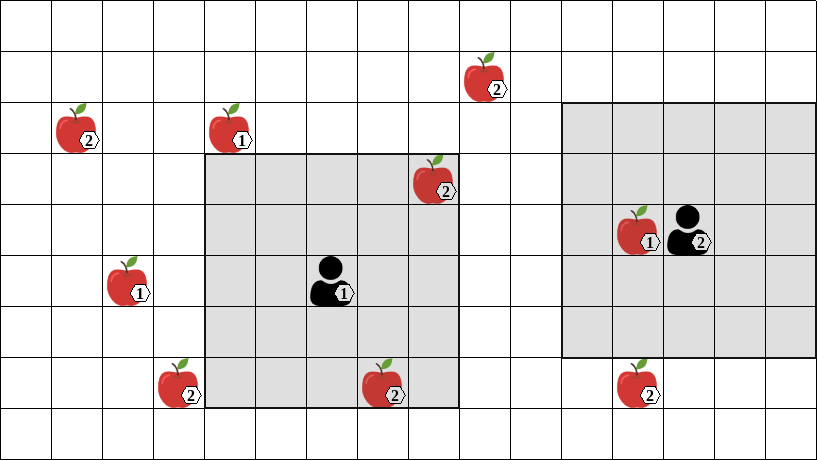
\includegraphics[width = \linewidth]{images/environments/lbf/foraging_po.png}
        % \caption{Caption}
        % \label{fig:enter-label}
    \end{figure}
    \end{column}
    \end{columns}   
\end{frame}

\begin{frame}[t]{Single Agent Belief Update}

To simplify, let's consider the single-agent perspective:

\blist
    \item The initial belief state is given by $b_{i}^0 = \mu$
    \item After taking action \(a_{i}^t\) and observing \(o^{t+1}_i\), the belief state \(b_{i}^t \) is updated to \(b_{i}^{t+1} \) using a Bayesian update:
\elist
\vspace{-1.0em}

\visible<1->{
    \[
        b_{i}^{t+1}(s') \propto \sum_{s \in S} b_{i}^{t}(s) \mathcal{T}(s'|s, a^{t}_i) \mathcal{O}_i (o^{t+1}_{i}|a^{t}_{i}, s')
    \]
}
\vspace{-1.0em}

\visible<2->{
    In MARL this type of update is typically \fat{infeasible}:
    \blist
        \item High-dimensional state spaces make storage and updates of beliefs intractable
        \item In MARL for POSG, agents assumed not to know $(S, \mathcal{T}, \mathcal{O}_i)$
        \item Deep learning can be used to approximate state information (see later lectures)
    \elist
}

\end{frame}

\section{Modeling Communication}

\begin{frame}{Modeling Communication}

\begin{columns}
\begin{column}{0.4\textwidth}
    \begin{figure}
        \centering
        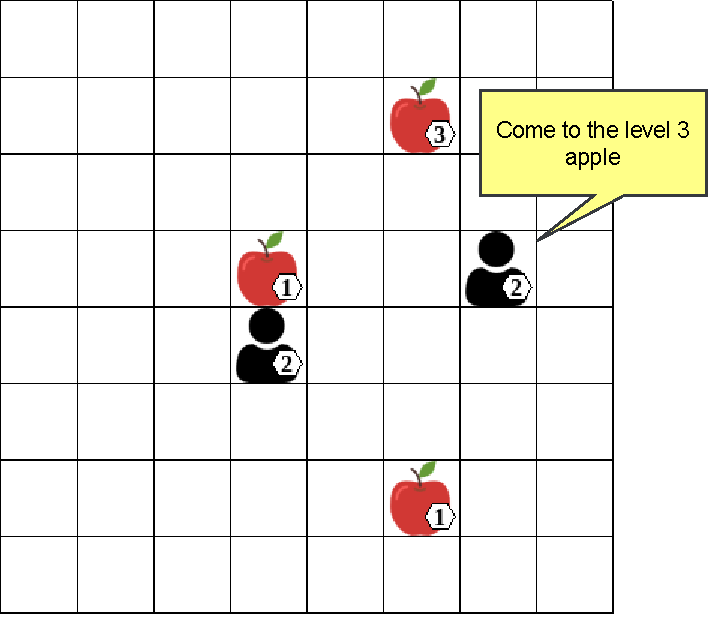
\includegraphics[width = \linewidth]{images/chapter_3/communication_example.pdf}
        % \caption{Caption}
        % \label{fig:enter-label}
    \end{figure}
\end{column} 

\begin{column}{0.6\textwidth}
\blist
    \item Using games, we can model more complex agent interactions, such as communication 
    \item We can view communication as a type of action that other agents can observe without affecting the state of the environment
    \item Agents learn communication meanings through trials and observations, identical to environment actions
    \item This can lead to the evolution of a shared language or protocol
\elist
\end{column}
\end{columns}
\end{frame}

\begin{frame}{Communication Actions}

To model communication, we can extend the action set of agents:

\begin{equation*}
    A_i = X_i \times M_i
\end{equation*}

\blist
    \item Where \(M_i\) is a set of possible messages \(\{m1, m2, m3, ...\}\) and \(X_i\) is the set of environment actions
    \item The action \(a_i\) can thus be expressed as \((x_i, m_i) \in A_i\)
\elist
    
\end{frame}

\begin{frame}{Communication in Stochastic Games}
    \blist
        \item Agents observe the current state \( s_t \) and previous joint action \( a_{t-1} \) 
        \item Communication action \( m_{t-1}^i \) by agent \( i \) is part of \( a_{t-1} \) and observed by all agents
        \item State transitions are independent of the joint communication actions \( M = \times_{i \in I} M_i \)
    \elist
    \begin{equation*}
        \forall s, s' \in S \forall a \in A, m \in M : T(s'|s, a) = T(s'|s, \langle(a_{1}, m_{1}), \ldots, (a_{n}, m_{n})\rangle)
    \end{equation*}
\end{frame}

\begin{frame}{Communication in POSG}

    \blist
        \item In POSG we can use the observation function \(\mathcal{O}_i\) to model noisy or unreliable communication
        \item We can define the observation as \(o_{i}^{t} = [\bar{s}^t, w^{t-1}_{1}, ..., w^{t-1}_{n}]\)
        \blist
            \item \(\bar{s}^t\) is some partial information about the state 
            \item \(w_{j}^{t-1}\) is a message from the agent \(j\) at time step \(t-1\) which has been augmented by \(\mathcal{O}_i\)
            \item E.g. \(w_{j}^{t-1} = f(m_{j}^{t-1})\) where \(f(m_{j}^{t-1}) = m_{j}^{t-1} + \eta\), and \(\eta\) is some random noise component.
        \elist
        \item You could also model $\mathcal{O}_i$ to hide messages such that $w^{t-j}_{1} = \emptyset$  if agent $i$ is too far from agent $j$
    \elist
    
\end{frame}

\section{Assumptions in Games}

\begin{frame}{Game Theory Assumption}

    \blist
        \item  In game theory, we typically assume that all agents know all components of the game \fat{(complete knowledge games)}
        \item Agents know all agents' \fat{action spaces and reward functions}
        \item Knowledge of other agents' reward functions may be used for informing the agent's \fat{best response} action (we will cover this in more depth in the next lecture)
        \item Knowledge of the transition function (\( T \)) allows for predicting state changes and \fat{planning} actions multiple steps ahead
    \elist
    
\end{frame}

\begin{frame}{MARL Assumptions}

\blist
    \item In MARL, we assume \fat{limited knowledge}, i.e. no knowledge of transition function $\mathcal{T}$ and no knowledge of agents' reward functions $\Rew_i$
    \item Additional assumption can be added and specific knowledge of the game can be held\fat{ mutually} or \fat{asymmetrically }
    \item We usually assume the \fat{number of agents to be fixed}, although recent research has looked at \textit{open} multi-agent systems, this will not be covered in these lectures 
\elist

\end{frame}

\begin{frame}{Dictionary: Reinforcement Learning \(\leftrightarrow\) Game Theory}
\centering

\begin{columns}[T]
    \begin{column}{0.5\textwidth}
        \fbox{
        \begin{tabular}{ccc}
        \fat{RL} & & \fat{GT} \\
        \hline
        environment & $\leftrightarrow$ & game \\
        agent & $\leftrightarrow$ & player \\
        reward & $\leftrightarrow$ & payoff, utility \\
        policy & $\leftrightarrow$ & strategy \\
        deterministic X & $\leftrightarrow$ & pure X \\
        probabilistic X & $\leftrightarrow$ & mixed X \\
        joint X & $\leftrightarrow$ & X profile \\
        \end{tabular}
        }
        \vspace{5pt}
        \blist
            \item \fat{Environment/Game}: Model with actions, observations, rewards, state dynamics.
            \item \fat{Agent/Player}: Decision-maker, possibly with specific roles.
        \elist
    \end{column}


    \begin{column}{0.5\textwidth}
        \blist
            \item \fat{Reward/Payoff, Utility}: Scalar value received after an action
            \item \fat{Policy/Strategy}: Assigns probabilities to actions; 'pure strategy' may refer to actions
            \item \fat{Deterministic X/Pure X}: Assigns probability 1 to $X$ e.g. $X$ = equilibrium or policy
            \item \fat{Probabilistic X/Mixed X}: Assigns probabilities $\leq 1$ to $X$
            \item \fat{Joint X/X Profile}: Tuple representing collective aspects, e.g., rewards or policies
        \elist
    \end{column}
\end{columns}
\end{frame}

\begin{frame}{Summary}

\fat{We covered:}
    \blist
        \item Game models 
        \item Modelling agent communication
        \item Assumptions of game models
    \elist

\fat{Next we'll cover:}

    \blist
        \item Solution concepts for games
    \elist

    
\end{frame}


\end{document}

